\documentclass{article}

%https://tex.stackexchange.com/questions/36109/making-tikz-nodes-hyperlinkable
\usepackage[hidelinks]{hyperref}
\usepackage{tikz}
\usetikzlibrary{decorations.pathreplacing,shapes,arrows,positioning}
\usetikzlibrary{calc, chains}
\begin{document}
\tikzset{
    hyperlink node/.style={
        alias=sourcenode,
        append after command={
            let     \p1 = (sourcenode.north west),
                \p2=(sourcenode.south east),
                \n1={\x2-\x1},
                \n2={\y1-\y2} in
            node [inner sep=0pt, outer sep=0pt,anchor=north west,at=(\p1)] {\hyperref[#1]{\XeTeXLinkBox{\phantom{\rule{\n1}{\n2}}}}}
                    %xelatex needs \XeTeXLinkBox, won't create a link unless it
                    %finds text --- rules don't work without \XeTeXLinkBox.
                    %Still builds correctly with pdflatex and lualatex
        }
    }
}

%\tikz \node [draw, inner sep=2ex,hyperlink node=Sect] {Go to Page Two};

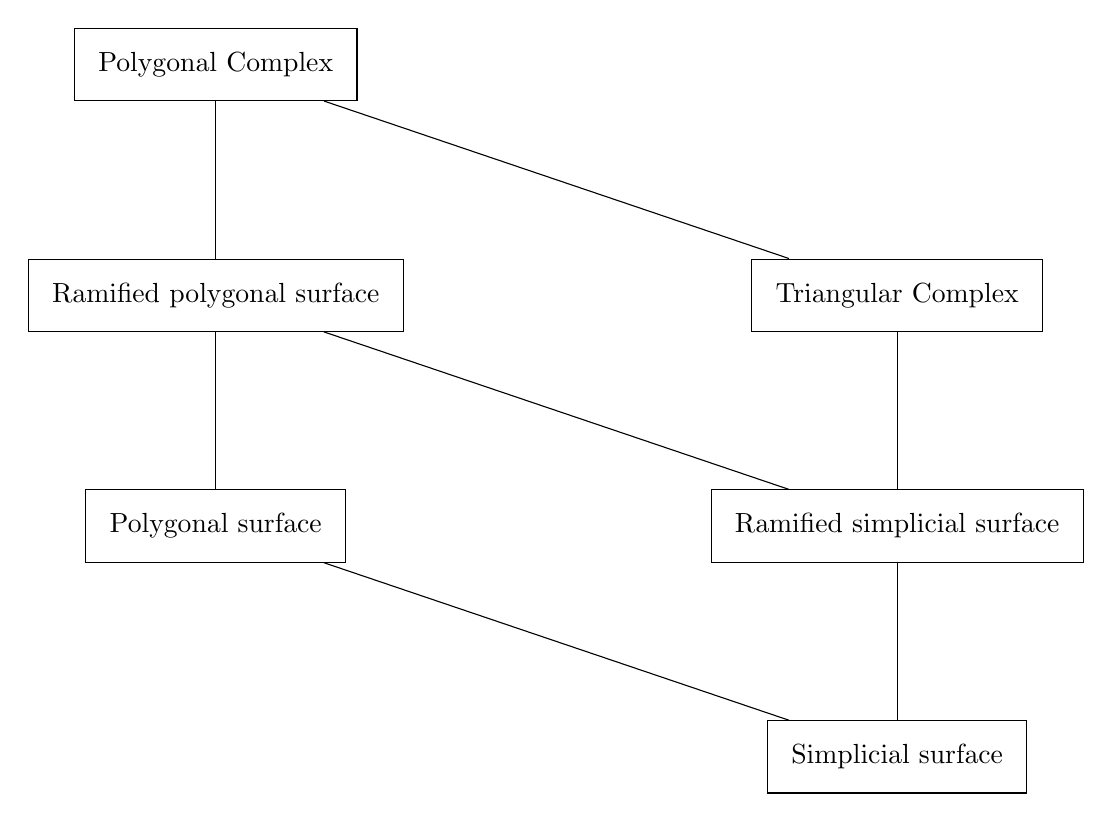
\begin{tikzpicture}[start chain, every node/.style={on chain,join}, node distance=2cm and 5cm, box/.style={
% The shape:
rectangle,
% The size:
inner sep=2ex,
% The border:
draw=black
}]



	\node (PC) [box] {Polygonal Complex};
	\begin{scope}[start branch=triangle]
		\node (TC) [box, below right=of PC] {Triangular Complex};
		\node (RSS) [box, below=of TC] {Ramified simplicial surface};
	\end{scope}

	\node (RPS) [box, below=of PC, join=with chain/triangle-end] {Ramified polygonal surface};
	
	\node (PS) [box, below=of RPS] {Polygonal surface};
	\node (SS) [box, below=of RSS, join=with chain/triangle-end] {Simplicial surface};
\end{tikzpicture}


\clearpage
\section{Abschnitt}\label{Sect}
\end{document} 